% !TEX TS-program = pdflatex
% !TEX encoding = UTF-8 Unicode

\documentclass[UTF8, a4paper, 12pt]{report}
	\title{模式识别作业\\——Bayesian分类器}
	\author{姓名学号}
	\date{2020/12/15}

\usepackage{ctex}
\usepackage{amsmath}
\usepackage{amssymb}
\usepackage{titlesec} % set Chapter1 to chinese 第一章
\usepackage{zhnumber}
\titleformat{\chapter}{\raggedright\Huge\bfseries}{第\,\zhnum{chapter}\,章}{1em}{}
 \usepackage{indentfirst} % 首行缩进
\usepackage{enumitem} % 序号
\usepackage{graphicx} % 插图
\makeatletter
\newcommand*\bigcdot{\mathpalette\bigcdot@{.5}}
\newcommand*\bigcdot@[2]{\mathbin{\vcenter{\hbox{\scalebox{#2}{$\m@th#1\bullet$}}}}}
\makeatother

\usepackage{bm}
\usepackage{float}
\usepackage{tikz} % 流程图
\usetikzlibrary{shapes, arrows}
\tikzstyle{startstop} = [rectangle,rounded corners, minimum width=3cm,minimum height=1cm,text centered, draw=black,fill=red!30]
\tikzstyle{io} = [trapezium, trapezium left angle = 70,trapezium right angle=110,minimum width=3cm,minimum height=1cm,text centered,draw=black,fill=blue!30]
\tikzstyle{process} = [rectangle,minimum width=3cm,minimum height=1cm,text centered,text width =3cm,draw=black,fill=orange!30]
\tikzstyle{decision} = [diamond,minimum width=3cm,minimum height=1cm,text centered,draw=black,fill=green!30]
\tikzstyle{arrow} = [thick,->,>=stealth]

\usepackage{dirtree} % 目录树绘制

\usepackage{fancyhdr} % use this package to set page
\pagestyle{fancy}
\lhead{}
\rhead{}
\chead{\leftmark} % set all the headings in the center of the page
\lfoot{}
\rfoot{}
\cfoot{\thepage}
\renewcommand{\headrulewidth}{0pt} % set off the line over the heading

% \usepackage[left=2.50cm, right=2.50cm, top=2.50cm, bottom=2.50cm]{geometry} % page distance
\usepackage[top=2.50cm, bottom=2.50cm]{geometry}


\begin{document}
% \CJKindent
\maketitle % generate the document title
\thispagestyle{empty} % this page with no page number
\clearpage % create a new page

\pagestyle{plain} % set the content with no heading, but a page number
\setcounter{page}{1} % set the content page as Page I
\pagenumbering{Roman} % set the I(Roman)
\tableofcontents % generate the content
\clearpage

\pagestyle{fancy} % the main body use fancy
\setcounter{page}{1} % set the main body page as Page 1
\pagenumbering{arabic} % set the 1(arabic)

\chapter{实验目的}
	\section{实验要求}
		设计并实现一个基于最小错误率贝叶斯方法的手写数字识别系统,并实现以下功能:
		\begin{enumerate}[itemindent=1em]
			\renewcommand{\labelenumi}{\theenumi)}
			\item 搭建平台;(确定编程环境,构建实验平台框架)
			\item 特征描述;
			\item 建立基于最小错误率的贝叶斯决策分类器;
			\item 实现手写数字识别
		\end{enumerate}

	\section{实验思路}
		整个实验要求搭建一个手写数字识别系统,故总体来说需要实现三个模块:用户交互界面(GUI)模块、特征提取与处理模块、监督学习算法训练与识别模块。以下几章将从如上所述几个方面分别展开。总体实验框架如图1.1所示。

	\section{实验意义}
		通过设计手写数字识别系统,深入理解模式识别的总体框架、特征提取和各种算法,对模式识别这一方向有更深入的理解,对自动化与人工智能整体方向有更深入的理解。在工程实现的过程中,加强代码能力和解决问题的能力。
		\begin{figure}
			\centering
			\begin{tikzpicture}[node distance=2cm]
				\node (start) [startstop] {Start};
				\node(ui) [startstop, below of=start]{GUI};
				\node (write) [io, below of=ui] {手写数字};
				\node (selection) [decision, below of=write, yshift=-0.75cm] {训练识别};
				\node (save) [process, right of=selection, xshift=3cm] {保存图片};
				\node (recog) [process, below of=selection, yshift=-0.75cm] {识别};
				\node (train) [process, right of=recog, xshift=3cm] {算法训练};
				\node (end) [startstop, below of=recog] {End};
	     
				%连接具体形状
				\draw [arrow](start) -- (ui);
				\draw [arrow](ui) -- (write);
				\draw [arrow](write) -- (selection);
				\draw [arrow](selection) -- node[anchor=south]{save}(save);
				\draw [arrow](save) --(train);
				\draw [arrow](save) |- (ui);
				\draw [arrow](selection) -- node[anchor=east]{recognize}(recog);
				\draw [arrow](train) -- (recog);
				\draw [arrow](recog) -- (end);

			\end{tikzpicture}
			\caption{总体实验框架(流程图)}
			\label{fig:1.1}
		\end{figure}


\clearpage

\chapter{实验平台}
	\section{编程环境}
		鉴于个人对python语言的了解较其他语言丰富,故在实现过程中,采用python作为主要使用的编程语言,在pycharm平台上进行GUI设计。设计过程中所使用的语言、编程环境及主要依赖库的详细信息如表2.1:
		\begin{table}[!h]
		\centering
		\caption{实验环境信息}  
		\begin{tabular*}{13cm}{lll}  
		\hline  
		名称 & 版本  & 描述 \\  
		\hline  
		\hline
		python  & 3.7.9 & 编程语言 \\  
		pycharm  & community-2020.2 & 集成开发环境(编程、调试、运行) \\  
		PyQt5 & 5.15.1 & GUI设计\\
		PyTorch & 1.6.0+cpu & 数学运算及算法实现\\  
		Torchvision & 0.7.0+cpu & 数据特征处理\\
		PIL & 7.2.0 & 图片读取和特征处理\\
		\hline  
		\end{tabular*}  
		\end{table}  

	\section{平台搭建}
		\subsection{PyQt5简介}
			PyQt5是基于Digia公司强大的图形程式框架Qt5的python接口,由一组python模块构成。PyQt5本身拥有超过620个类和6000函数及方法。在可以运行于多个平台,包括:Unix, Windows, and Mac OS。\\
			PyQt5有自己的图形界面,也有封装在python里的内嵌库,在这里,为了与我们的算法融合,我们选用PyQt5内嵌于python的库。PyQt5分为很多模块,主要模块有:
			\begin{enumerate}[itemindent=1em]
				\renewcommand{\labelenumi}{•}
				\item QtCore 包含了核心的非GUI的功能。主要和时间、文件与文件夹、各种数据、流、URLs、mime类文件、进程与线程一起使用。
				\item QtGui 包含了窗口系统、事件处理、2D图像、基本绘画、字体和文字类。
				\item QtWidgets 包含了大多数GUI设计需要的工具、插件和窗体,是在Qt中创建用户界面的主要元素。
				\item QtMultimedia
			\end{enumerate}

		\subsection{画板实现}
			画板是用户交互的主要界面,其作用是实现手写数字的输入和读取,涉及到的插件和工具有:QWidget、QPixemap、QPainter、QPoint、QPen、QMouse等,其作用如表2.2所示。
			\begin{table}[!h]
			\centering
			\caption{画板设计所涉及相关插件及工具介绍}  
			\begin{tabular*}{13cm}{lll}  
			\hline  
			名称 & 描述 \\  
			\hline  
			\hline
			QWidget  & 作为画板设计的窗口 \\  
			QPixemap  & 用于图片的读写与显示 \\  
			QPainter & 作画工具(画笔的外壳)\\
			QPoint & 鼠标位置与画板位置获取\\  
			QPen & 画笔(内部属性)\\
			QMouse & 获取鼠标动态\\
			\hline  
			\end{tabular*}  
			\end{table}  
		
			如图2.1所示,使用画布可以实现手写板功能。用户通过鼠标在画板上写数字,画板记录并保存手写数字,用于算法训练和识别。
			\begin{figure}[H]
			\centering
			
\includegraphics[scale=0.5]{./img/PaintBoard.eps}
			\caption{画布界面展示}
			\label{fig:2.1}
			\end{figure}

		\subsection{GUI实现}
			将前述画布作为一个插件布局到一个较大QWidget窗口之中,利用QLabel、QTextEdit、QLineEdit、QCheckBox、QIcon等等实现整体GUI布局,如图2.2所示。再在该窗口外面套一层QMainWindow制成的窗体,形成最终的应用窗口。
			\begin{figure}[H]
			\centering
			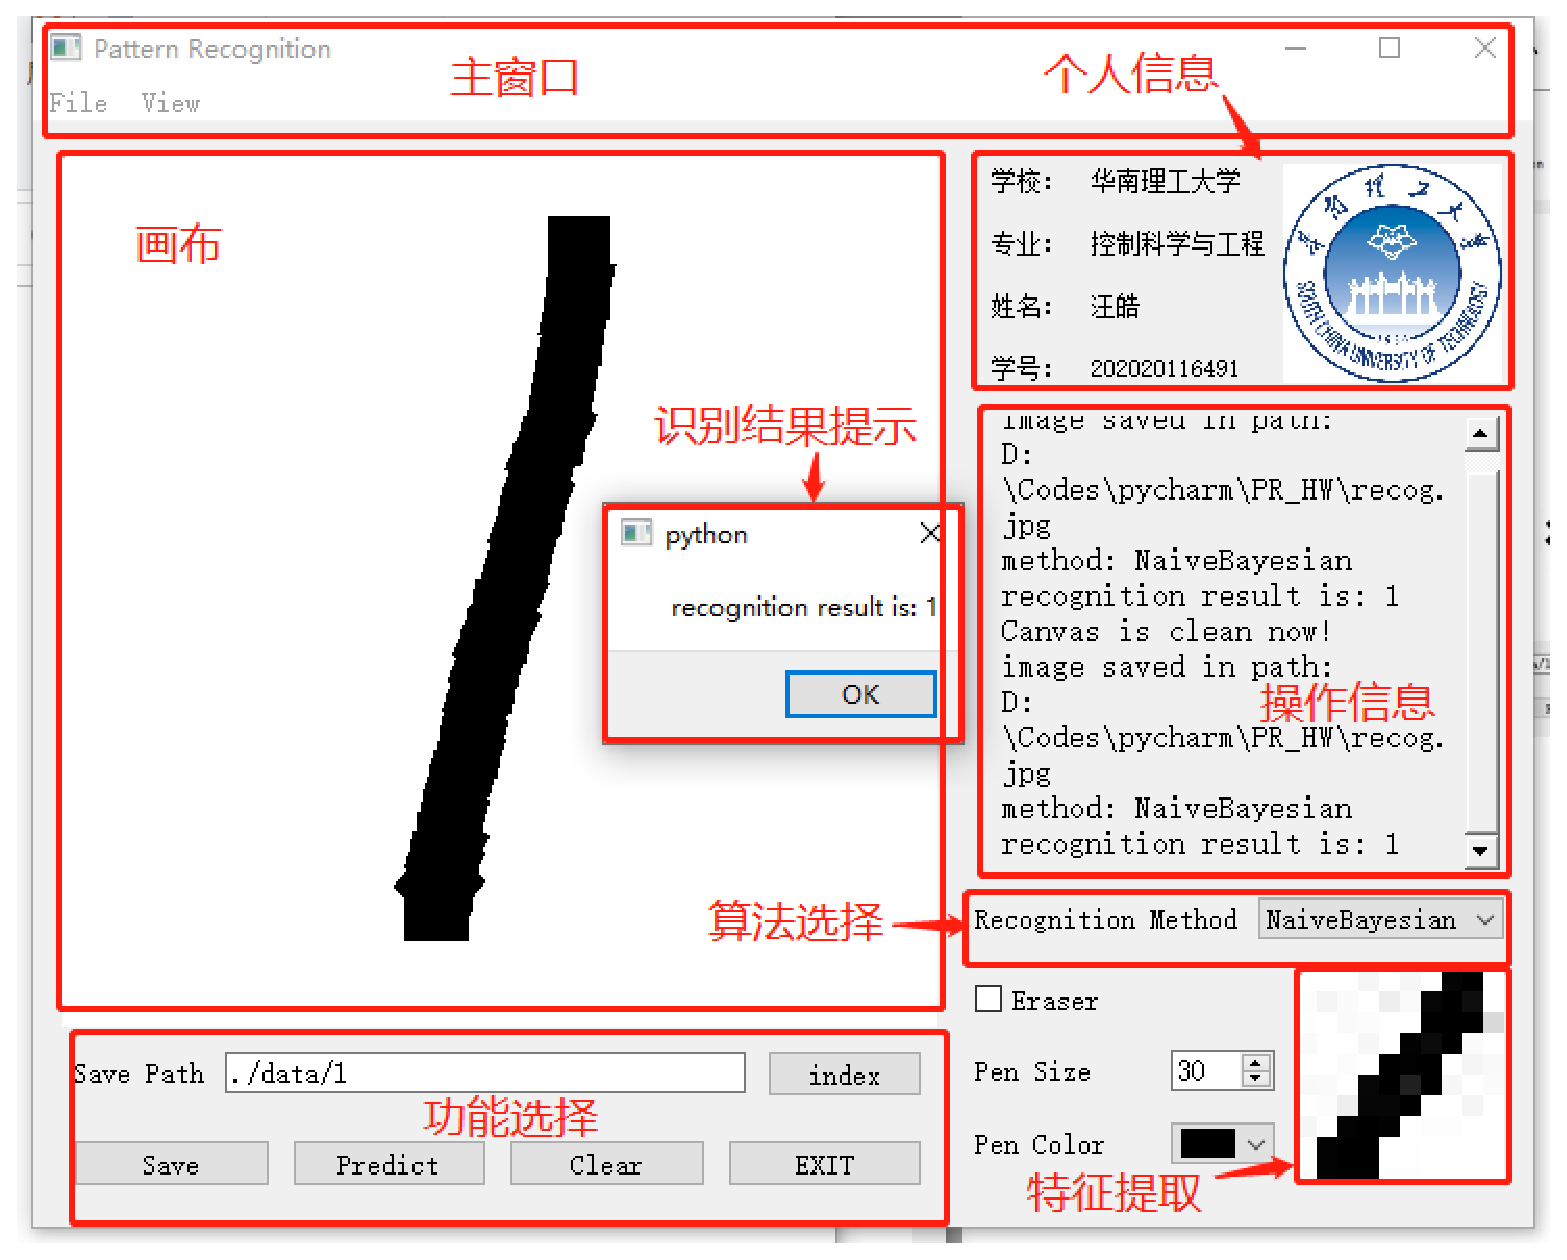
\includegraphics[scale=0.5]{./img/GUI.eps}
			\caption{GUI界面展示}
			\label{fig:2.2}
			\end{figure}	
\clearpage
\chapter{数据集}
	\section{数据集}
		利用GUI的画布手写数字,分为训练集和测试集,并按数字名存到文件夹中,文件目录如下所示。其中,训练集中每个数字有20张图片,测试集中每个数字有10张图片。
		\begin{figure}[!h]
			\centering
			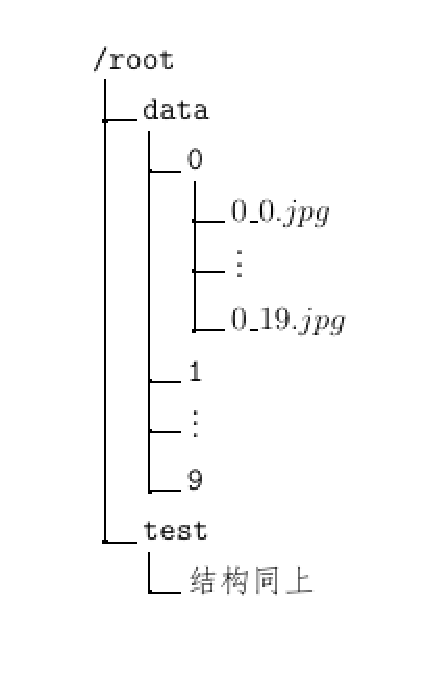
\includegraphics[scale=0.8]{./img/DataDirTree.eps}
			\caption{数据集文件目录}
			\label{fig:3.1}
		\end{figure}

	\section{特征处理}
		\subsection{目的}
			物理和结构上的特征通常易于为人的直觉感知,但有时难以定量描述,因而不易用于机器判别。而数学上的特征易于用机器定量描述和判别,故通常使用数学特征作为模式识别任务的特征描述,例如基于统计的特征。

			但对于一幅图像而言,例如我们的手写数字图像,尺寸是420*420,即使不考虑色彩,也至少有17万多个像素值作为原始特征。而每一个特征点的取值从0-255共有256个取值可能。原始这一幅图几十万的像素特征样本分布很稀疏,高维特征计算量大、冗余性高,且不能反映对象的本质。因而,特征处理的一个重要任务或目的就是从如此繁多的特征中选择其中的重要特征以减少特征数量,同时尽量保留分类信息。

		\subsection{处理方法}
			通常能够提取有效信息、压缩特征空间的特征处理方法有:特征提取和特征选择。所谓特征提取是用映射或变换的方法把原始特征变换为较少的新特征。而特征选择是指从原始特征中挑选出一些最有代表性、分类性能最好的特征。
		
			为了采用朴素贝叶斯实现的最小错误率贝叶斯分类器, 我们希望最后的特征满足以下条件:
			\begin{enumerate}[itemindent=1em]
				\renewcommand{\labelenumi}{\theenumi)}
				\item 每个特征之间尽量独立分布;
				\item 特征用一维数组表示;
				\item 特征取值尽量少;
				\item 特征数组维数尽量小。
			\end{enumerate}

			于是,我们将图像有效范围从420*420的像素阵中分割出来,按均值滤波缩小到10*10,再转换成二值图,并展开成一维数组,最后得到一个尺寸为1*100维的特征数组,其中间过程如图3.2所示。
			\begin{figure}[!h]
			\centering
			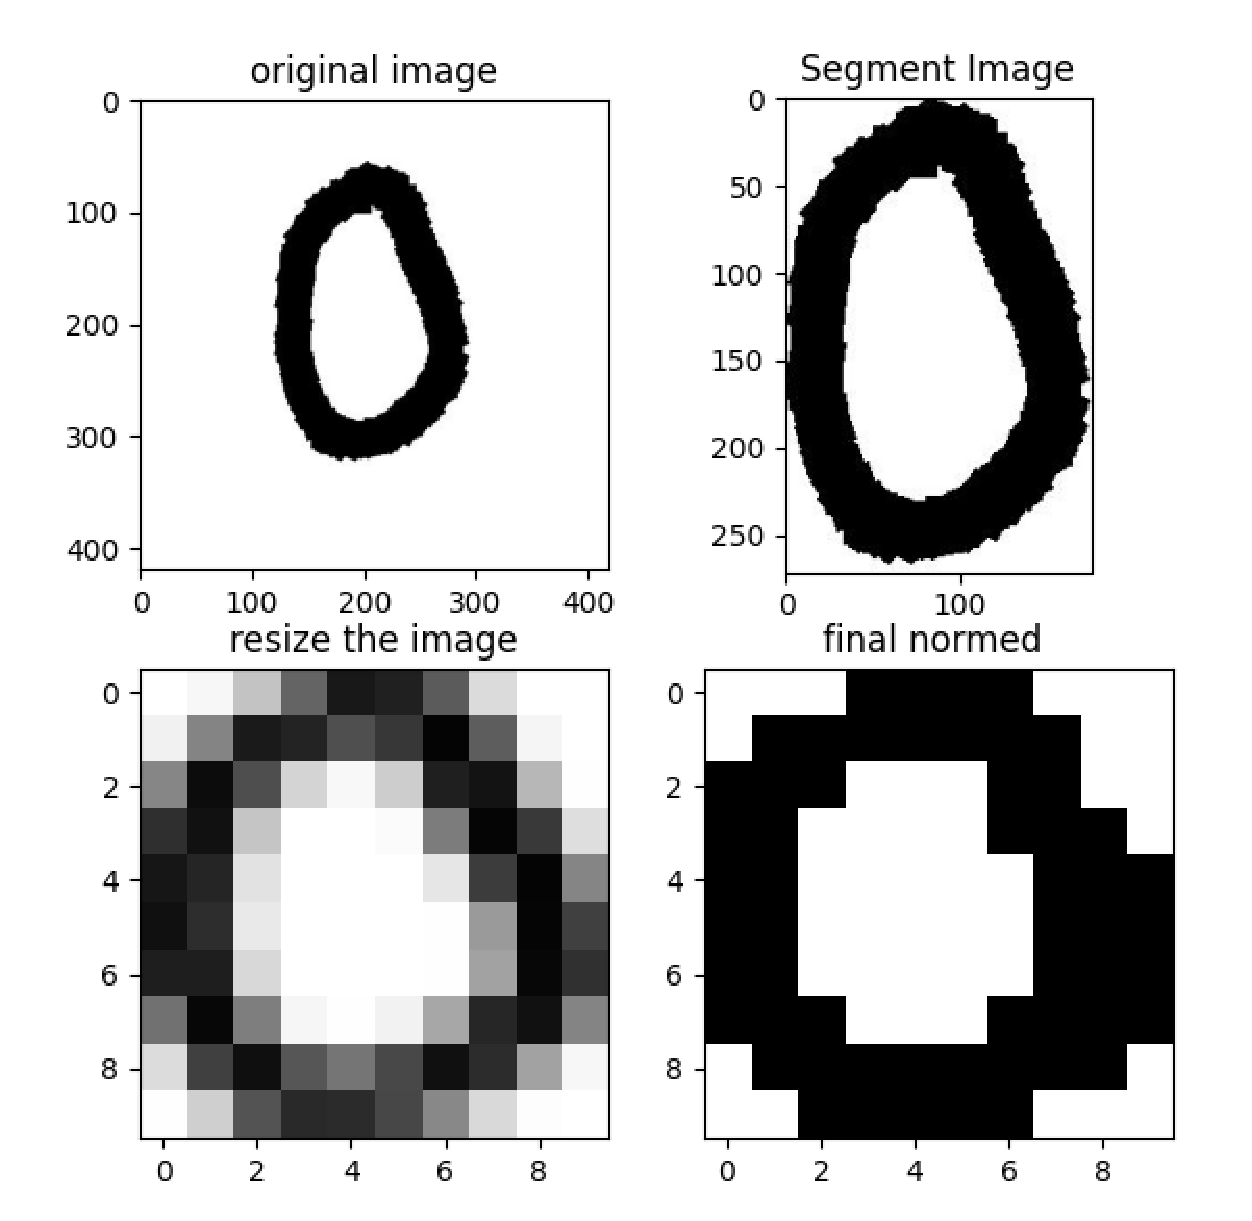
\includegraphics[scale=0.35]{./img/FeatureMapping.eps}
			\caption{特征处理过程}
			\label{fig:3.2}
			\end{figure}
\clearpage

\chapter{Bayesian分类器}
	\section{贝叶斯决策}
			贝叶斯决策论是概率框架下实施决策的基本方法,对分类任务来说,在所有相关概率都已知的理想情形下,贝叶斯决策论考虑如何基于这些概率和误判损失函数来选择最优的类别标记。
		\subsection{贝叶斯定理}
			贝叶斯决策基于贝叶斯定理。在讨论贝叶斯定理之前,我们讨论下以下概率及公式。
			\begin{enumerate}[itemindent=1em]
				\renewcommand{\labelenumi}{\theenumi)}
				\item 联合概率:指两个独立事件 $A$ 和事件 $B$ 同时发生的概率。联合概率可表示为 $P(AB)$ ;
				\item 条件概率:指事件 $A$ 在事件 $B$、$C$、$\cdots$ 发生的条件下发生的概率。条件概率表示为 $P(A|B, C, \cdots)$ 。对于两个事件 $A$ 和 $B$ ,其计算公式为:
					\begin{equation}
						P(A|B) = \frac{P(AB)}{P(B)}
					\end{equation}
				\item 全概率公式:全概率公式将一复杂事件 $B$ 的概率求解问题转化为了在不同情况下发生的简单事件的概率的求和问题。即如果事件 $A_1$、$A_2$、$\cdots$、$A_n$ 构成一个完备事件组(两两互不相容且和为全集),且有 $P(A_i)>0$,则对任一事件 $B$ 有如下公式:
					\begin{equation}
						P(B) = P(B|A_1) \bigcdot P(B|A_2) \bigcdot  \cdots  \bigcdot P(B|A_n)
					\end{equation}
或
					\begin{equation}
						P(B) = \sum_{i=1}^{n} P(A_i)P(|B|A_i)
					\end{equation}
			\end{enumerate}

			贝叶斯定理由英国数学家贝叶斯提出,用于描述两个条件概率之间的关系,对于两个事件 $A$ 和 $B$,其计算公式为:
			\begin{equation}
				P(AB) = P(A|B)P(B) = P(B|A)P(A)
			\end{equation}
其中,$p(A)$是 $A$ 的先验概率(边缘概率);$P(A|B)$ 是已知 $B$ 发生后 $A$ 发生的条件概率,称为 $A$ 的后验概率;其余同理。

		\subsection{贝叶斯决策论}
			在贝叶斯决策中,我们考虑以上概率模型。假设一个分类任务中有 $N$ 种可能的类别标记,即 $\mathcal{Y} = {c_1, c_2, \cdots, c_N}$,$\lambda_{ij}$ 是将一个真实标记为 $c_j$ 的样本误分类为 $c_i$ 所产生的损失。基于后验概率 $P(c_i|x)$ 可获得将样本 $\bm{x}$ 分类为 $c_i$ 所产生的期望损失,即在样本 $\bm{x}$ 上的“条件风险”:
			\begin{equation}
				R(c_i|\bm{x}) = \sum_{j=1}^{N} {\lambda_{ij} P(c_j|\bm{x})}
			\end{equation}
于是贝叶斯决策的任务即是寻找一个判定准则 $h: \mathcal{X} \mapsto \mathcal{Y}$以最小化总体风险
			\begin{equation}
				R(h) = \mathbb{E} _{\bm{x}} [R(h(\bm{x})|\bm{x}]
			\end{equation}
从而,贝叶斯准则只需选择使得条件风险 $R(c|\bm{x})$ 最小的类别标记即可。

			故而,结合前述贝叶斯定理和全概率公式,可以得到贝叶斯分类器的一般公式为:					\begin{equation}
				P(c_i|\bm{x})=\frac{P(c_i)P(\bm{x}|c_i)}{P(\bm{x})}=\frac{P(c_i)P(\bm{x}|c_i)}{\sum_{j=1}^{N}{P(c_j)P(\bm{x}|c_j)}}
			\end{equation}

	\section{朴素贝叶斯}
		\subsection{原理}
			对于式4.7,其涉及到三个代估计变量 $P(c_i)$、$P(\bm{x}|c_i)$ 和 $P(\bm{x})$。其中, $P(c_i)$ 的估计可直接从样本类别信息中得到。而 $P(\bm{x})$ 的估计实际上可由 $P(\bm{x})=\sum_{j=1}^{N}{P(c_j)P(\bm{x}|c_j)}$ 所确定。因而最终的估计重点落在了后验概率$P(\bm{x}|c_i)$ 上。对于该概率,朴素贝叶斯采用了“属性条件独立性假设”, 即假设所有属性相互独立。且对于所有类别来说, $P(\bm{x})$ 不改变,故而,朴素贝叶斯判定准则为:
			\begin{equation}
				c^* = \mathop{\arg\min}_{c \in \mathcal{Y}} {P(c)\prod \limits_{i=0}^n {P(x_i|c)}}
			\end{equation}

			若令 $D_c$表示训练集 $D$中第 $c$ 类样本组成的集合,若有充足的独立同分布样
本,则可容易地估计出类先验概率
			\begin{equation}
				P(c) = \frac{|D_c|}{|D|}
			\end{equation}
若令 $D_{c, x_i}$ 表示 $D_c$ 中在第 $i$ 个属性上取值为 $x_i$ 的样本组成的集合,则条件概率 $P(x_i|c)$ 可估计为
			\begin{equation}
				P(x_i|c) = \frac{|D_{c, x_i}|}{|D_c|}
			\end{equation}

			故而,最终的贝叶斯判定准则可写为
			\begin{equation}
				c^* = \mathop{\arg\min}_{c \in \mathcal{Y}} {\frac{|D_c|}{|D|} \prod \limits_{i=0}^n {\frac{|D_{c, x_i}|}{|D_c|}}}
			\end{equation}

		\subsection{设计}
			借由上一节的讨论,$P(\bm{x})=\sum_{j=1}^{N}{P(c_j)P(\bm{x}|c_j)}$ 对于某个确定的样本 $\bm{x}$ 一般不变,故在分类器设计时,我们将这一项做归一化处理。且我们的手写数字数据集各类别分布较为均匀,故而类先验概率 $P(c)$ 对于每一类都相等,故这一项亦可去掉。

			而对于另两项,考虑到实际问题中,可能存在这种情况:某个属性值在训练集中没有与某个类同时出现过。这时,若再按前述式4.11进行判别将出现分子某一项为 $0$ 的情况。此时,由于分子是连乘,则最终结果,无论其他属性再好,最终的结果都是0,这样的预测不是我们想看到的,所以我们对式中的概率进行拉普拉斯修正,如下所示:
			\begin{equation}
				P(c) = \frac{|D_c|+1}{|D|+N}
			\end{equation}
			\begin{equation}
				P(x_i|c) = \frac{|D_{c, x_i}|+1}{|D_c|+N_i}
			\end{equation}
其中,$N_i$ 表示第 $i$ 个属性可能的取值数(在手写数字识别任务中,均取10。

		\subsection{实现}
			基于最小错误率的朴素贝叶斯分类器是由python实现的。

			朴素贝叶斯分类器涉及到两个针对数据集的量,一个是用于分类的后验概率,另一个是用于估计后验概率的各个特征上的类条件概率,其他两个概率由于对于所有数据集都一样,故直接做归一化处理。

			我们将训练集中按前述特征提取后的数据依据类别分类存入数组,在预测新样本时,分别计算每一个类别对应的类条件概率。计算时使用 $pytorch$ 的 $tensor$ 进行计算,使用 $CPU$ 加速。在计算最终的类条件概率时,由于式4.11中连乘的结果使得最后的类条件概率过小,故而在这里对每一个特征对应的条件概率所计算出的结果取对数 $torch.log()$,然后将连乘变成连加,这样结果就不会下溢出。

	\section{算法评价}
		为了评价我们的系统,我们取测试集的所有图片进行预测,然后计算其 $top1$ 和 $top5$ 准确率分别为 $98\%$ 和 $100\%$。可见,我们的算法准确率比较高。
\clearpage

\chapter{实验结果与结论}
		我们将保存的算法模型导入 $GUI$ 对应的预测函数中,进行测试,如图5.1所示。当选择了NaiveBayes作为预测算法进行预测,在正常书写时均能准确预测出正确结果,并能在 $GUI$ 右下角反映出特征提取后的可视化图形。而预测结果及其他信息则能通过右边的信息框反映出来,同时预测结果以弹窗的形式反映。
		\begin{figure}[!h]
		\centering
		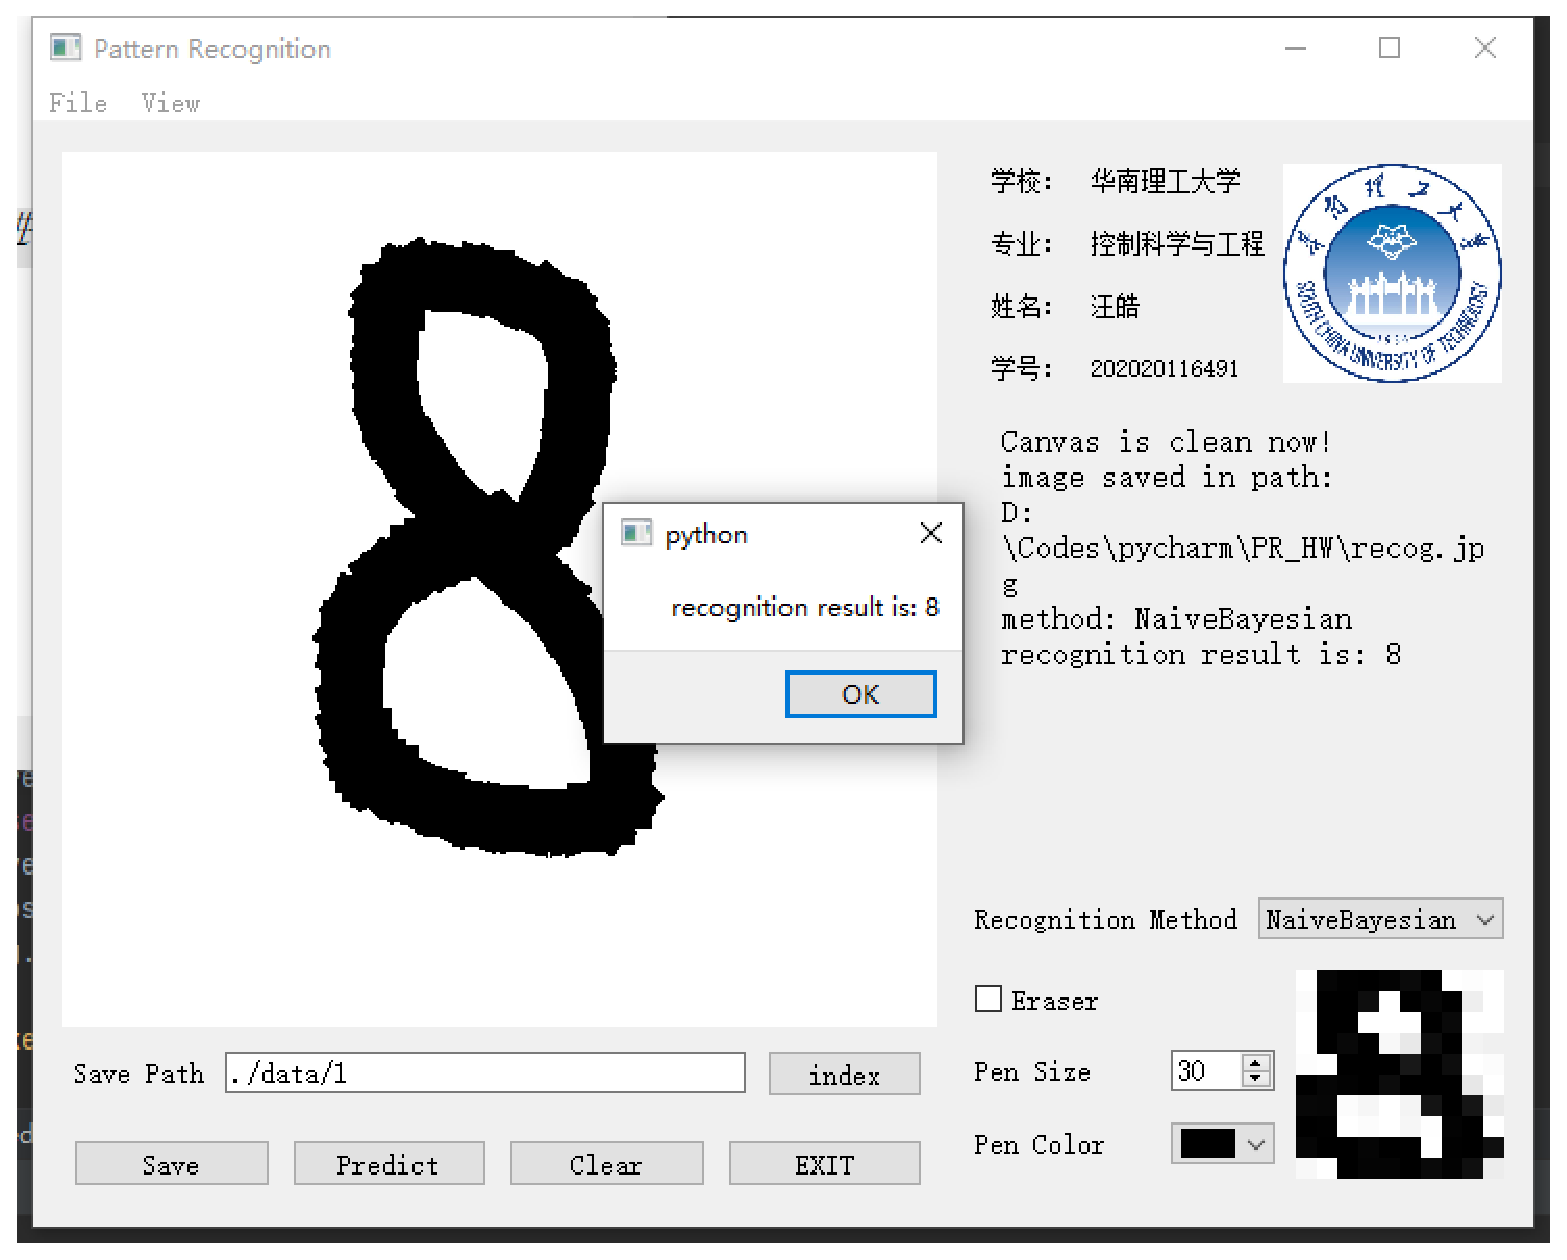
\includegraphics[scale=0.5]{./img/Predict.eps}
		\caption{预测结果展示}
		\label{fig:5.1}
		\end{figure}

		经过多次测试,发现所设计的基于最小错误率的朴素贝叶斯分类器能够很好地完成手写数字分类任务,且准确率能够达到 $98\%$。
\clearpage
\end{document}